\title{Assignment 1: CS 763}
\author{
  Sai Charith \\ 160050083
  \and
  Sanchit\\ 160050043  
  \and
  Mayank\\ 160050039 
}

\documentclass[a4paper]{article}
\usepackage{amsmath}

\usepackage{amsfonts,amssymb,amsthm}
\usepackage[margin=0.94in]{geometry}
\usepackage{graphicx}
\begin{document}
\maketitle
%\makebox[\linewidth]{\rule{\paperwidth}{0.4pt}}
%\noindent\rule{12cm}{0.4pt}
\hrulefill
\\
\textbf{Problem 5a:} \\
Let R represent rotation, translation matrix and K represent camera internals and A be the direction of parallel linse passing through B and C. Any points on these lines can be represented as $P=tA+B$ , $Q=sA+C$ respectievely. So these points correspond to KRP and KRQ respectievely. Since R just rotates or transforms the lines still remain parallel. So RP and RQ correspond to $P' = t'A'+B'$ and $Q'=s'A'+C'$. Now as t' and s' tends to infinity, in the image they correspond to their respective vanishing points.\\
Therefore, 

\begin{equation*}
\begin{split}
&\implies |x_i- \mu| \leq \sqrt{\sum_{j=1}^{n} (x_j-\mu)^2 } \quad for\; any\; i\\
& \;\;\;\qquad KP' = K(t'A'+B')\\
&\implies KP' = K(A'+\frac{B'}{t'}) \qquad (Homogenous\;\; Coordinates)\\ 
&\implies KP' = KA' \qquad (as \;\;t'\rightarrow\varpropto)\\
&\qquad \;\; KP' = KA' \qquad (Similarly\;\; for\;\; Q)\\
\end{split}
\end{equation*}
As, 
\[
K=
\begin{bmatrix}
    c       & cs & x_{H}  \\
    0       & c(1+m) & y_{H}  \\
    0       & 0 & 1
\end{bmatrix}
\]
the parallel lines vanish only if [0 0 1].A$'$ is not 0. (If it is 0 they vanish at infinity)\\ \\
\textbf{Problem 5b:}\\
Let ($x_1L+A_1$, $x_2L+A_2$), ($y_1M+B_1$, $y_2M+B_2$), ($z_1N+C_1$, $z_2N+C_2$) be the three sets of co-planer parallel lines after applying the R transformation.\\
Let K be the matrix representing internals of camera.\\
As the lines are coplaner $L.(M \times N) = 0 $  ie, where $L = [l_1,l_2,l_3]^T$, $M = [m_1,m_2,m_3]^T$, $N = [n_1,n_2,n_3]^T$
\[
Q=
\begin{bmatrix}
    l_1       & l_2 & l_3  \\
    m_1       & m_2 & m_3  \\
    n_1       & n_2 & n_3  \\
\end{bmatrix}
\]

\begin{equation*} 
\begin{split}
& det(Q) = 0 \\
\implies & det(Q^T)=0 \\
\implies & det(KQ^T)=0\\
\implies & det(K[L\; M\; N]) =0 \\
\implies & det([KL\;\; KM\;\; KN]) = 0\\
\end{split}
\end{equation*}
$\implies$ area of triangle formed by KL, KM, KN (vanishing points) is zero. So the vanishing points of the three sets of coplaner parellel lines are collinear. 


\hrulefill\\


\textbf{\newline Problem 6:}

\begin{figure}[h!]
 \centering
\caption{Picture with pixel values}
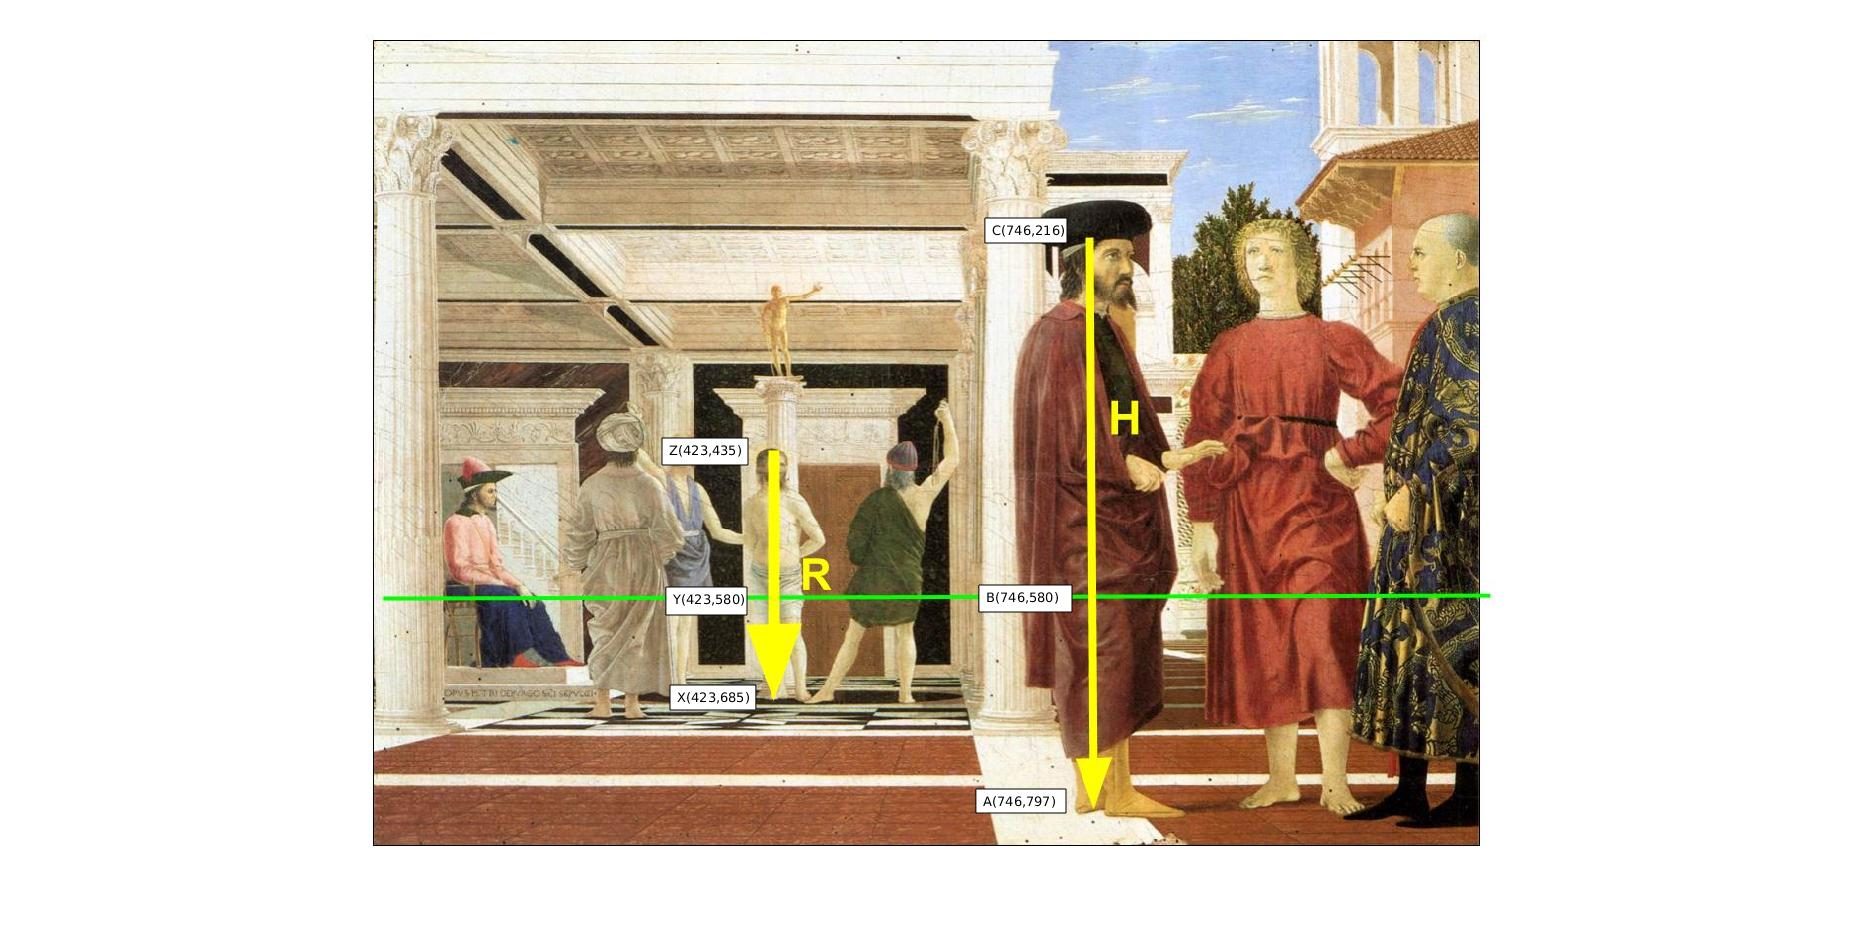
\includegraphics[width=1\textwidth]{Q6/measuredpicture.jpg}
\end{figure}

In the image the lines in y-direction do not vanish(as they are perpendicular to the axis of the image). So the line AC extended vanishes at infinity say at D. Similarly XZ vanishes at W. Let P' denote point P in world co-ordinates.

Using cross ratios we have

\begin{equation*} 
\begin{split}
 \frac{AC*BD}{AD*BC} &= \frac{A'C'*B'D'}{A'D'*B'C'} \\
\implies  \frac{AC}{BC} &=  \frac{A'C'}{B'C'} \\
\implies  \frac{AC-AB}{AC} &=  \frac{A'C'-A'B'}{A'C'} \\
\implies \frac{AB}{AC} &=  \frac{A'B'}{A'C'} \quad \textit{(equation 1)} \\
 \end{split}
\end{equation*}
Similarly
\begin{equation*} 
\begin{split}
 \frac{XZ*YW}{XW*YZ} &= \frac{X'Z'*Y'W'}{X'W'*Y'Z'} \\
\implies  \frac{XZ}{YZ} &=  \frac{X'Z'}{Y'Z'} \\
\implies  \frac{XY}{XZ} &=  \frac{X'Y'}{X'Z'} \quad \textit{(equation 2)}\\
 \end{split}
\end{equation*}
Now if we draw line passing through B and Y it coincides with horizon. This says that the line should be parallel to both sky and ground in the world co-ordinates. This says $ A'B' = X'Y' $ (Assuming both persons are on same horizontal level) . Now dividing the equations 1 and 2 we have
 
\begin{equation*}
\begin{split}
\frac{AB*XZ}{AC*XY} &= \frac{X'Z'}{A'C'} \\
\implies A'C' &= X'Z' \frac{AC*XY}{AB*XZ} \\
\end{split}
\end{equation*}
From the pixel values of the points we have  
\begin{equation*}
\begin{split}
A'C' &= 180\times\frac{(797-216)\times(685-580)}{(797-580)\times(685-435)} \\
\implies A'C' &= 202 cm
\end{split}
\end{equation*}
So, the hieght of the person in the image is 202 cm.


\hrulefill \\


\textbf{Problem 4:}
\\
(a)-\\
\indent Since there is no correlation between car being behind a door
and a participant choosing a door so no matter $Z1$ occured or not $C_i$ will remain $\frac{1}{3}$ for $1\leq i \leq3$.i.e.\\
$$P(C_1|Z_1)=\frac{1}{3} $$
$$P(C_2|Z_1)=\frac{1}{3} $$
$$P(C_3|Z_1)=\frac{1}{3} $$
\begin{center}
  $\clubsuit$~$\clubsuit$~$\clubsuit$
\end{center}
(b)-\\
\indent We know that the host is intelligent and (s)he is always going to open a door not chosen by the contestant, and is also going to open a door behind which there is a stone. Now considering the given question:-\\\\
$P(H_3|C_1,Z_1)$ :- This means the probability that the host opens door 3 provided the car is behind door 1 and contestant chose door 1. So here since the car is behind 1 and contestant has chosen door 1 then door 2 and 3 both have stones behind it and the host can open any one of them with equal probability, hence:-
$$P(H_3|C_1,Z_1)=\frac{1}{2}$$
$P(H_3|C_2,Z_1)$ :- This means the probability that the host opens door 3 provided the car is behind door 2 and contestant chose door 1.So here since contestant has chosen door 1 and car is behind door 2 the host does not have any other option other than door 3.Hence:-
$$P(H_3|C_2,Z_1)=1$$
$P(H_3|C_3,Z_1)$ :- This means the probability that the host opens door 3 provided the car is behind door 3 and contestant chose door 1.So here since contestant has chosen door 1 and car is behind door 3 the host does not have any other option other than door 2.So (s)he cant open door 3.Hence:-
$$P(H_3|C_3,Z_1)=0$$
\begin{center}
  $\clubsuit$~$\clubsuit$~$\clubsuit$
\end{center}
(c)-\\
\indent To find $P(C_2|H3,Z_1)$ we have the formula
$$P(C_2|H3,Z_1)=\frac{P(H_3|C_2,Z_1)P(C_2,Z_1)}{P(H_3,Z_1)}$$
Now $P(H_3|C_2,Z_1)$ is already calculated to be 1 in previous part\\
Also $Z_1$ and $C_2$ are independent events with probability of each being $\frac{1}{3}$,hence
\begin{equation*}
\begin{split}
P(C_2,Z_1)&=P(C_2)P(Z_1)\\
&=\frac{1}{3}.\frac{1}{3}\\
&=\frac{1}{9}
\end{split}
\end{equation*}
Now $P(H_3,Z_1)$ means the probability that the contestant chooses door 1 and the host opens door 3.Here 3 separate cases have to be considered i.e.\\
\indent case 1:Car is behind door 1 i.e.\\
$$P(H_3,Z_1|C_1)=P(H_3|C_1,Z_1)=\frac{1}{2}$$
\indent case 2:Car is behind door 2 i.e.\\
$$P(H_3,Z_1|C_2)=P(H_3|C_2,Z_1)=1$$
\indent case 3:Car is behind door 3 i.e.\\
$$P(H_3,Z_1|C_3)=P(H_3|C_3,Z_1)=0$$
Each of the following cases are equally likely with probability $\frac{1}{3}$,hence:-\\
\begin{equation*}
\begin{split}
P(H_3,Z_1)&=P(C_1)P(H_3,Z_1|C_1)+P(C_2)P(H_3,Z_1|C_2)+P(C_3)P(H_3,Z_1|C_3)\\
&=\frac{1}{3}.\frac{1}{2}+\frac{1}{3}.1+\frac{1}{3}.0\\
&=\frac{1}{6}+\frac{1}{3}\\
&=\frac{1}{2}
\end{split}
\end{equation*}
Putting in the equation we have
\begin{equation*}
\begin{split}
P(C_2|H_3,Z_1)&=\frac{1.\frac{1}{9}}{\frac{1}{2}}\\
&=\frac{\frac{1}{9}}{\frac{1}{2}}\\
&=\frac{2}{9}\\
\end{split}
\end{equation*}
\begin{center}
  $\clubsuit$~$\clubsuit$~$\clubsuit$
\end{center}
(d)-\\
\indent To find $P(C_1|H3,Z_1)$ we have the formula
$$P(C_1|H3,Z_1)=\frac{P(H_3|C_1,Z_1)P(C_1,Z_1)}{P(H_3,Z_1)}$$
Now $P(H_3|C_1,Z_1)$ is already calculated to be $\frac{1}{2}$ in previous part\\
Also $Z_1$ and $C_1$ are independent events with probability of each being $\frac{1}{3}$,hence
\begin{equation*}
\begin{split}
P(C_1,Z_1)&=P(C_1)P(Z_1)\\
&=\frac{1}{3}.\frac{1}{3}\\
&=\frac{1}{9}
\end{split}
\end{equation*}
Now $P(H_3,Z_1)$ means the probability that the contestant chooses door 1 and the host opens door 3.Here 3 separate cases have to be considered i.e.\\
\indent case 1:Car is behind door 1 i.e.\\
$$P(H_3,Z_1|C_1)=P(H_3|C_1,Z_1)=\frac{1}{2}$$
\indent case 2:Car is behind door 2 i.e.\\
$$P(H_3,Z_1|C_2)=P(H_3|C_2,Z_1)=1$$
\indent case 3:Car is behind door 3 i.e.\\
$$P(H_3,Z_1|C_3)=P(H_3|C_3,Z_1)=0$$
Each of the following cases are equally likely with probability $\frac{1}{3}$,hence:-\\
\begin{equation*}
\begin{split}
P(H_3,Z_1)&=P(C_1)P(H_3,Z_1|C_1)+P(C_2)P(H_3,Z_1|C_2)+P(C_3)P(H_3,Z_1|C_3)\\
&=\frac{1}{3}.\frac{1}{2}+\frac{1}{3}.1+\frac{1}{3}.0\\
&=\frac{1}{6}+\frac{1}{3}\\
&=\frac{1}{2}
\end{split}
\end{equation*}
Putting in the equation we have
\begin{equation*}
\begin{split}
P(C_1|H_3,Z_1)&=\frac{\frac{1}{2}.\frac{1}{9}}{\frac{1}{2}}\\
&=\frac{1}{9}\\
\end{split}
\end{equation*}
\begin{center}
  $\clubsuit$~$\clubsuit$~$\clubsuit$
\end{center}
(e)-\\
Switching is actually beneficial and increases chances of winning by a factor of 2. If we do not switch then the probability is $\frac{1}{9}$ and if we do it is indeed$\frac{2}{9}$\\
\begin{center}
  $\clubsuit$~$\clubsuit$~$\clubsuit$
\end{center}
\hrulefill \\
\textbf{Problem 5:}

Probability that a person speaks only language p\textsubscript{i} is 
 (since the ability to speak different languages is independent)
$$ (1-p_1)(1-p_2)...p_i...(1-p_n) $$

If we consider that a person speaks only a p\textsubscript{i} this rules out the possibility that he speaks another language. So the events that such a person speaks either p\textsubscript{i} or p\textsubscript{j} are mutually exclusive. So required probability is
$$ p_1(1-p_2)(1-p_3)...(1-p_n)+(1-p_1)p_2(1-p_3)...(1-p_n)+...+(1-p_1)(1-p_2)...(1-p_{n-1})p_n$$

\hrulefill \\ 
\newpage
\textbf{Problem 6:}
\graphicspath{ {/home/charith/Desktop/} }

%\begin{figure}[h!]
% \centering
%\caption{Corrupted values range from 5-10}
%\includegraphics[width=0.6\textwidth]{q61.png}
%\end{figure}
{\centering
Mean squared error=0.0013\qquad\qquad\qquad\qquad(Meadian filtering)\\
Mean squared error=0.0197\qquad\qquad\qquad\qquad(Mean filtering)\\
}
%\begin{figure}[h!]
%\centering
%\caption{corrupted values are range 100-120}
%\includegraphics[width=0.6\textwidth]{q62.png}
%\end{figure}
{\centering
Mean squared error=0.0013\qquad\qquad\qquad\qquad(Meadian filtering)\\
Mean squared error=3.6361\qquad\qquad\qquad\qquad(Mean filtering)\\
} 
\textbf{Observation:} It is clear from the mean squared error values and from plots that Moving Median Filtering is better than Moving Mean Filtering.

\textbf{Reason:} In the above plots the corrupted vales large compared to data values.So in case of Moving Mean Filtering all the points in neighbour-hood(-8,+8) have their mean affected because of this corrupted value.Hence the filtered value is far from original value by a significant amount.But in case of Moving Median filtering, the corrupted values go the ends(when sorted) median in the neighbourhood would generally be one among the values on the origianal curve resulting in less deviation from original curve.      
 
\hrulefill \\
\textbf{Problem 7:}
\begin{itemize}
\item newMean:

\qquad Let oldMean be $\mu$,newMean be $\mu_1$,new element be $x_{n+1}$,then
\begin{equation*}
\begin{split}
&\mu=\frac{\sum_{i=1}^{n}}{n} \qquad \qquad \qquad \qquad \\
&\implies \mu*n=\sum_{i=1}^{n}\\
But \; &\mu_1=\frac{\sum_{i=1}^{n}x_i+}{n+1}\\
& \implies \mu_1=\frac{\mu*n+x_{n+1}}{n+1}
\end{split}
\end{equation*} 
\qquad This formula is implipented on matlab to calculate newMean.
\item newMedian:

\qquad Let n be the number observations and d be the new data value, then

\qquad \qquad if n is odd 

\qquad \qquad \qquad if $d \geq oldMedian$

\qquad \qquad \qquad \qquad $NewMedian=avg(oldMedian,(min(d,x_{\frac{n+1}{2}+1}))$

\qquad \qquad \qquad else $NewMedian=avg(oldMedian,(min(d,x_{\frac{n-1}{2}}))$

\qquad \qquad else

\qquad \qquad\qquad if $ d\geq oldMedian$

\qquad \qquad\qquad \qquad $NewMedian=min(x_{\frac{n}{2}+1},d)$

\qquad \qquad\qquad else $NewMedian=max(x_{\frac{n}{2}},d)$

\qquad This is implemented as it is in Matlab to calculate NewMedian
\item newStd:

\qquad Let
\begin{itemize}
\item oldMean be $\mu$
\item newMean be $\mu_1$
\item new element be $x_{n+1}$
\item oldStd be $\sigma$
\item newStd be $\sigma_1$
\end{itemize}
\qquad then,
\begin{equation*}
\begin{split}
\sigma &=\sqrt{\frac{\sum_{i=1}^{n}(x_i-\mu)^2}{n-1}}\\
\implies \sigma^2(n-1)&={\sum_{i=1}^{n}[(x_i-\mu_1)+(\mu_1-\mu)]^2}\\
\implies \sigma^2(n-1) &={\sum_{i=1}^{n}\big[(x_i-\mu_1)^2+(\mu_1-\mu)^2+2((x_i-\mu_1)(\mu_1-\mu)\big]}\\
\implies \sigma^2(n-1) &={\sum_{i=1}^{n}(x_i-\mu_1)^2}+{\sum_{i=1}^{n}(\mu_1-\mu)^2}+{\sum_{i=1}^{n}2(x_i-\mu_1)(\mu_1-\mu)}\\
\implies \sigma^2(n-1)&={\sum_{i=1}^{n}(x_i-\mu_1)^2}+n(\mu_1-\mu)^2+2(\mu_1-\mu)^2{\sum_{i=1}^{n}(x_i-\mu_1)}\\
\implies \sigma^2(n-1)&+(x_{n+1}-\mu_1)^2=\sum_{i=1}^{n+1}(x_i-\mu_1)^2+n(\mu_1-\mu)^2+0\\\\
\implies \sigma^2(n-1)&+(x_{n+1}-\mu_1)^2=\sigma_1^2n+n(\mu_1-\mu)^2\\\\
\implies \sigma_1&=\sqrt{\frac{\sigma^2(n-1)+(x_{n+1}-\mu_1)^2-n(\mu_1-\mu)^2}{n}}\\
\end{split}
\end{equation*}

This formula was used to find newStd in matlab.function newStd = UpdateStd (OldMean, OldStd, NewMean, NewDataValue, A, n)
\end{itemize}

\hrulefill\\
\textbf{Problem 8:}\\
\\
The Input array is p:- 
$$p=[5,\, 10,\, 15,\, 20, \,30,\, 40, \,50,\, 60, \,70, \,80,\, 90,\, 95,\, 99,\, 99.99,\, 99.9999, \,100]$$
And the Output array n is:- 
$$n=[7,\, 10, \,12, \,14,\, 17, \,20,\, 23,\, 27,\, 30, \,35 ,\, 41,\, 47,\, 57,\, 80,\, 97,\, 366]$$

%\begin{figure}[h!]
% \centering
%\caption{probability \textit{vs} no. of people}
%\includegraphics[width=0.6\textwidth]{q8.png}
%\end{figure}
\hrulefill



\end{document}